\documentclass[12pt,letterpaper]{article}
\usepackage{graphicx,textcomp}
\usepackage{natbib}
\usepackage{setspace}
\usepackage{fullpage}
\usepackage{color}
\usepackage[reqno]{amsmath}
\usepackage{amsthm}
\usepackage{fancyvrb}
\usepackage{amssymb,enumerate}
\usepackage[all]{xy}
\usepackage{endnotes}
\usepackage{lscape}
\newtheorem{com}{Comment}
\usepackage{float}
\usepackage{hyperref}
\newtheorem{lem} {Lemma}
\newtheorem{prop}{Proposition}
\newtheorem{thm}{Theorem}
\newtheorem{defn}{Definition}
\newtheorem{cor}{Corollary}
\newtheorem{obs}{Observation}
\usepackage[compact]{titlesec}
\usepackage{dcolumn}
\usepackage{tikz}
\usetikzlibrary{arrows}
\usepackage{multirow}
\usepackage{xcolor}
\newcolumntype{.}{D{.}{.}{-1}}
\newcolumntype{d}[1]{D{.}{.}{#1}}
\definecolor{light-gray}{gray}{0.65}
\usepackage{url}
\usepackage{listings}
\usepackage{color}

\definecolor{codegreen}{rgb}{0,0.6,0}
\definecolor{codegray}{rgb}{0.5,0.5,0.5}
\definecolor{codepurple}{rgb}{0.58,0,0.82}
\definecolor{backcolour}{rgb}{0.95,0.95,0.92}

\lstdefinestyle{mystyle}{
	backgroundcolor=\color{backcolour},   
	commentstyle=\color{codegreen},
	keywordstyle=\color{magenta},
	numberstyle=\tiny\color{codegray},
	stringstyle=\color{codepurple},
	basicstyle=\footnotesize,
	breakatwhitespace=false,         
	breaklines=true,                 
	captionpos=b,                    
	keepspaces=true,                 
	numbers=left,                    
	numbersep=5pt,                  
	showspaces=false,                
	showstringspaces=false,
	showtabs=false,                  
	tabsize=2
}
\lstset{style=mystyle}
\newcommand{\Sref}[1]{Section~\ref{#1}}
\newtheorem{hyp}{Hypothesis}

\title{Problem Set 5}
\date{Due: March 4, 2020}
\author{QTM 200: Applied Regression Analysis}

\begin{document}
	\maketitle
	
	\section*{Instructions}
	\begin{itemize}
		\item Please show your work! You may lose points by simply writing in the answer. If the problem requires you to execute commands in \texttt{R}, please include the code you used to get your answers. Please also include the \texttt{.R} file that contains your code. If you are not sure if work needs to be shown for a particular problem, please ask.
		\item Your homework should be submitted electronically on the course GitHub page in \texttt{.pdf} form.
		\item This problem set is due at the beginning of class on Wednesday, March 4, 2020. No late assignments will be accepted.
		\item Total available points for this homework is 100.
	\end{itemize}
	
		\vspace{.5cm}
	
\noindent  Using the \texttt{teengamb} dataset, fit a model with \texttt{gamble} as the response and the other variables as predictors. 

\vspace{.5cm}
\lstinputlisting[language=R, firstline=41, lastline=43]{PS5.R}  
\newpage
Answer the following questions:
\vspace{.5cm}
\begin{enumerate}[(a)]
	 \item Check the constant variance assumption for the errors by plotting the residuals versus the fitted values.
	 
	 	\begin{figure} [h]
	 	\centering
	 	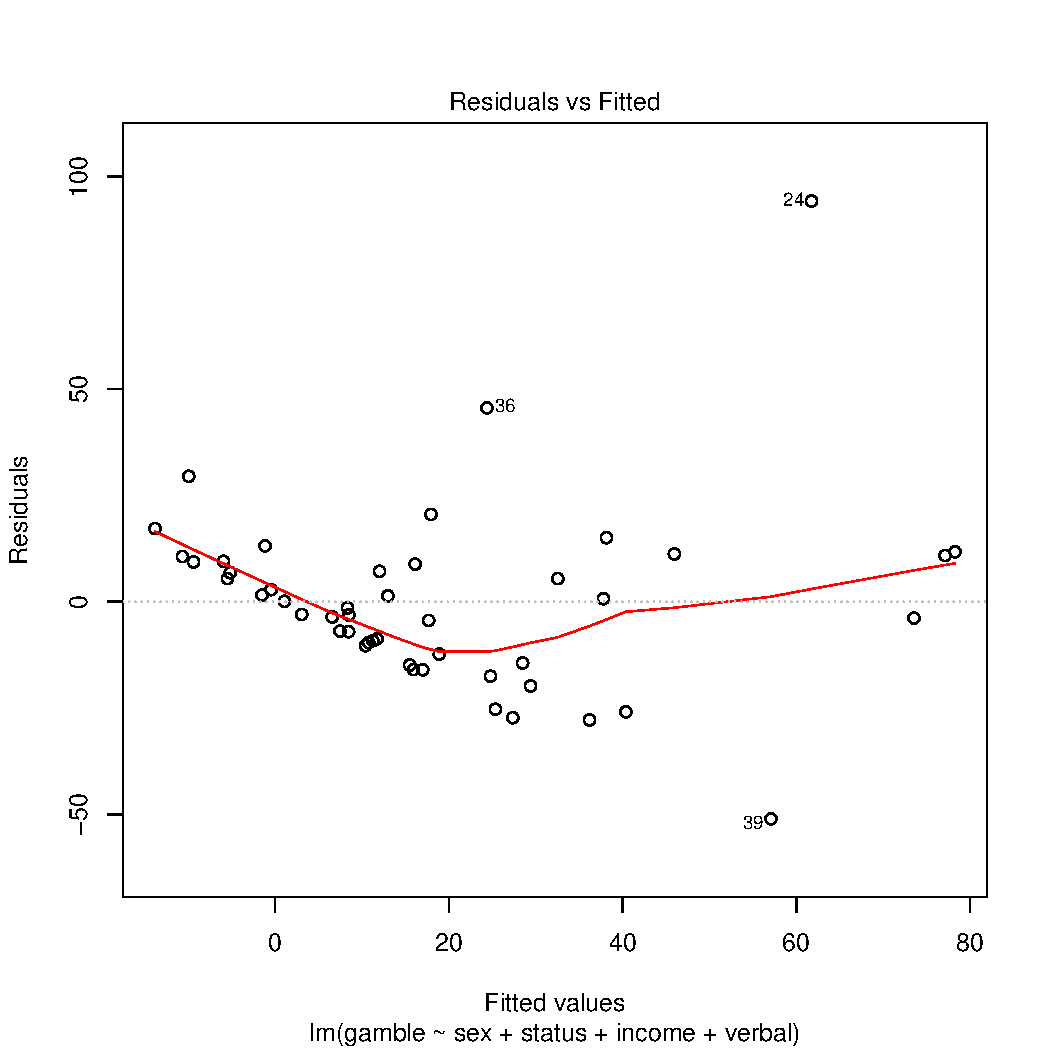
\includegraphics[width=0.7\linewidth]{plot1.pdf}
	 	\caption{Residuals vs. Fitted Values}
	 	\label{fig:graph2}
	 \end{figure}
 	\lstinputlisting[language=R, firstline = 49, lastline = 52]{PS5_Answers.R} 
 		
 Based on the plot of residuals against fitted values, the constant variance assumption doesn't seem to be met. The residuals fan out as the fitted values increase (especially the outliers after fitted value of 50), and there is no random scatter around the x-axis, some dipping below the horizontal line as fitted values increase.
 	
 	\newpage
	\item Check the normality assumption with a Q-Q plot of the studentized residuals.
	
		 	\begin{figure} [h]
		\centering
		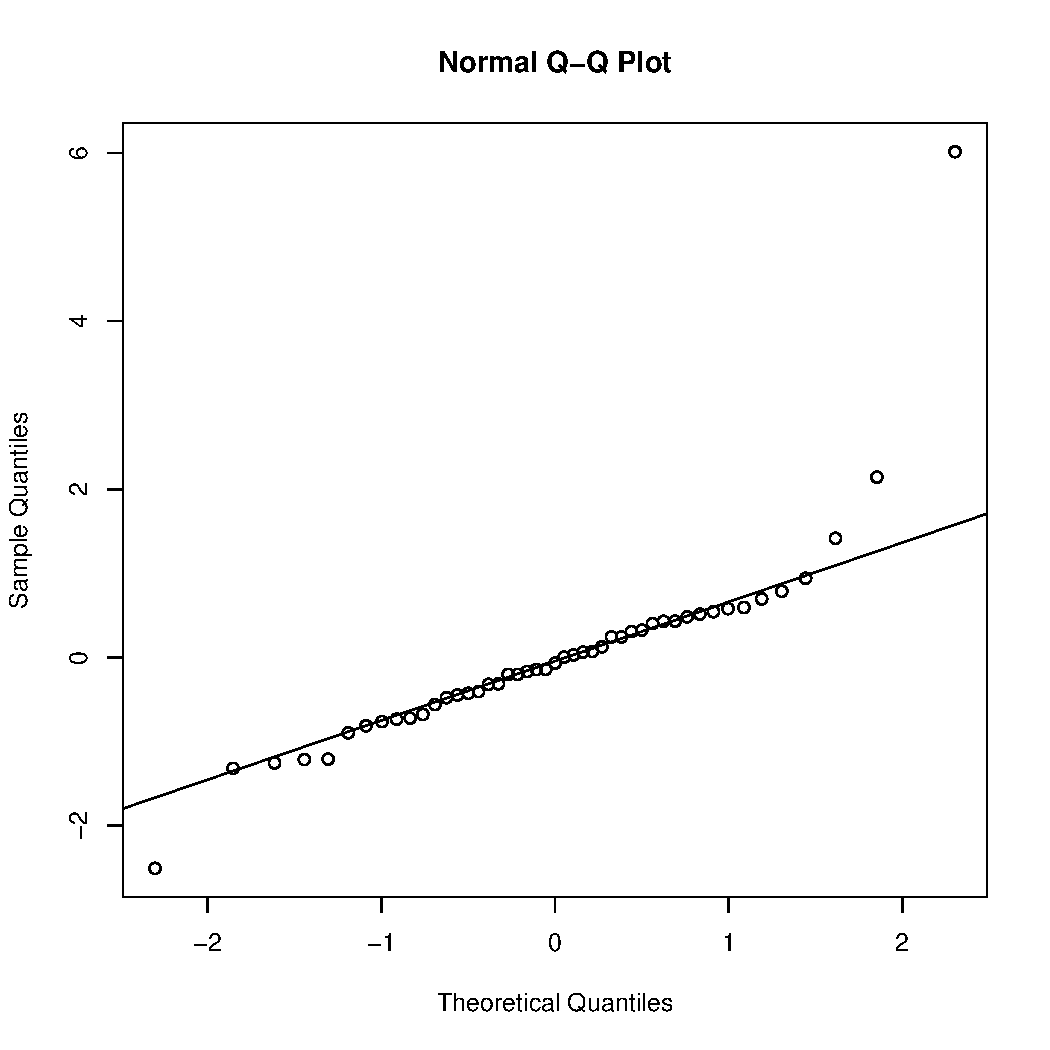
\includegraphics[width=0.7\linewidth]{plot2.pdf}
		\caption{Q-Q Plot of Studentized Residuals}
		\label{fig:graph2}
	\end{figure}
	
		 	\lstinputlisting[language=R, firstline = 62, lastline = 65]{PS5_Answers.R} 
		 	
Based on the Q-Q plot of the studentized residuals, the normality assumption is satisfied for the most part except for the outliers that occur as the theoretical quantiles increase. 

	 	
		\newpage
	\item Check for large leverage points by plotting the $h$ values.
	
	\begin{figure} [h]
		\centering
		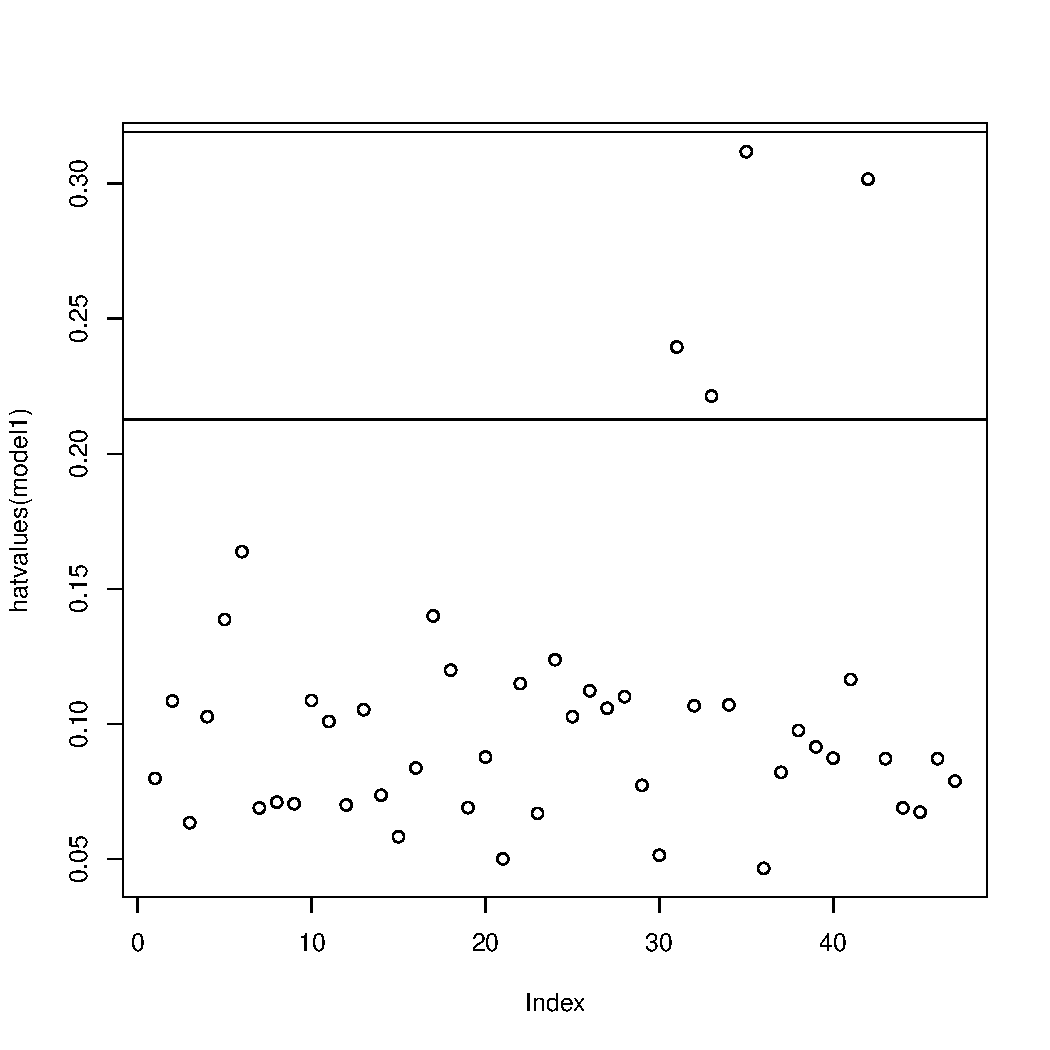
\includegraphics[width=0.7\linewidth]{plot3.pdf}
		\caption{Plot of Hat Values}
		\label{fig:graph2}
	\end{figure}
		 	\lstinputlisting[language=R, firstline = 71, lastline = 75]{PS5_Answers.R} 
		 	
The four points with higher hat values above the drawn line have high leverage, meaning that they have the potential to influence the fitted model. The lines were drawn based on the thresholds 2(k + 1) = n and 3(k + 1) = n, where k = number of predictors and n = sample size.

	\item Check for outliers by running an \texttt{outlierTest}.
			 	\lstinputlisting[language=R, firstline = 81, lastline = 81]{PS5_Answers.R} 
			 	
	Since the adjusted p-value (Bonferroni p) for the largest studentized residual is larger than 0.05 with a value of 0.76464, we would conclude that this model doesn't have any extreme residuals.
	
	\newpage
	\item Check for influential points by creating a "Bubble plot" with the hat-values and studentized residuals.
	
		\begin{figure} [h]
		\centering
		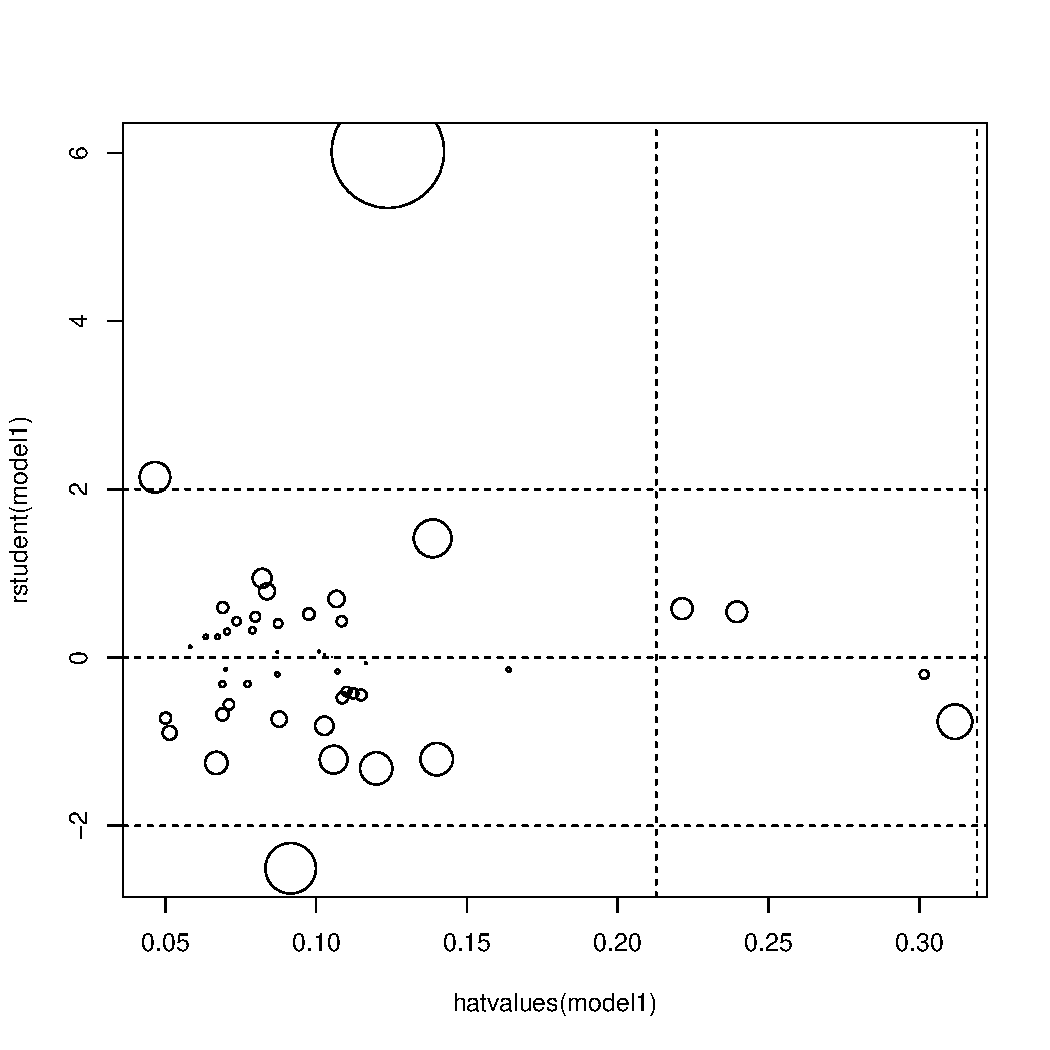
\includegraphics[width=0.7\linewidth]{plot4.pdf}
		\caption{Bubble Plot}
		\label{fig:graph2}
	\end{figure}

\item Check for outliers by running an \texttt{outlierTest}.
\lstinputlisting[language=R, firstline = 89, lastline = 96]{PS5_Answers.R} 

Based on the Bubble plot, there's an observation with a large studentized residual and a high Cook's distance, but with a low leverage. There are few observations with higher hat values/leverage, but with a small studentized residual/Cook's distance. The bubble plot shows that we do not have extreme outliers, since no observation has both a large studentized residual and high leverage/hat value. 
	% \item N/A.
\end{enumerate}

\end{document}
